% Source: src-8d14b1f9f511665ea10dbda45959a3b445a17806415be6b034f816bec663d7f5
% PDF SHA-256: 35e5d6f6bf052fcd9a2b91a1aa4215766fd4121425cfec7a62cfc4cdc7ab02a1
% PDF page 1, printed page 72, question 11. Shaded quadrilateral follows the printed inequalities.
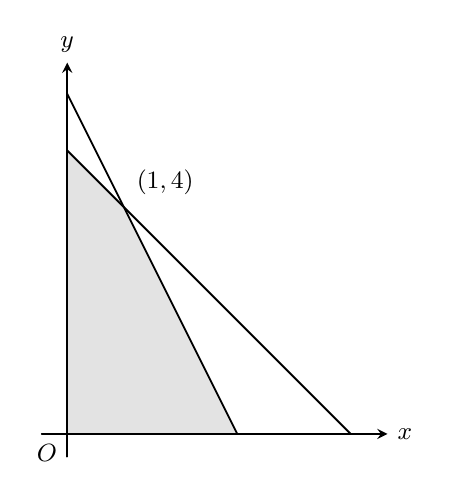
\begin{tikzpicture}[x=0.72cm,y=0.72cm,line cap=round,line join=round,line width=0.65pt,>=stealth,font=\small]
  \fill[gray!22] (0,0) -- (0,5) -- (1,4) -- (3,0) -- cycle;
  \draw[->] (-0.45,0) -- (5.65,0) node[right] {$x$};
  \draw[->] (0,-0.4) -- (0,6.55) node[above] {$y$};
  \draw (0,5) -- (5,0);
  \draw (0,6) -- (3,0);
  \node[below left] at (0,0) {$O$};
  \node[above right=1pt] at (1,4) {$(1,4)$};
\end{tikzpicture}
